% Slides for 2025-08-19
% To create a slide, use the following:
% \begin{frame}{TITLE}
%     BODY
% \end{frame}

% To create a slide with a bullet list, use the following:
% \begin{frame}{TITLE}
%     \begin{itemize}
%         \item ITEM 1
%         \item ITEM 2
%     \end{itemize}    
% \end{frame}

% To create a slide with numbered list, use the following:
% \begin{frame}{TITLE}
%     \begin{enumerate}
%         \item ITEM 1
%         \item ITEM 2
%     \end{enumerate}
% \end{frame}

% To create a slide with a graphic:
% 1. Add the graphic to this folder (named picture.png)
% 2. Use the following:
% \begin{frame}{TITLE}
%     \centering
%     \includegraphics[height=0.7\textheight,width=0.7\textwidth,keepaspectratio]{picture.png}
% \end{frame}

% To create a slide with two columns, use the following:
% \begin{frame}{TITLE}
%     \begin{columns}
%         \begin{column}{0.5\textwidth}
%             COLUMN 1 BODY
%         \end{column}
%         \begin{column}{0.5\textwidth}
%             COLUMN 2 BODY
%         \end{column}
%     \end{columns}
% \end{frame}


\begin{frame}{Summer Goal}
    \centering
    \begin{itemize}
        \item Classifying mangroves using Satellite
        \item Super-resolution from 10m/px to 1m/px
    \end{itemize}
\end{frame}

\begin{frame}{Testing Feasability}
    \centering
    \begin{enumerate}
        \item Problem Statement:
            \begin{itemize}
                \item What range of resolutions would be acceptable for the model?
            \end{itemize}
        \item Findings:
            \begin{itemize}
                \item We found that >0.5m/px gave bad classification metrics
                \item A super-resolution model would need to achieve <0.5m/px
            \end{itemize}
    \end{enumerate}
\end{frame}

\begin{frame}{Resampling Data}
    \centering
    We needed to test on various resolutions to check the model's tolerance.
    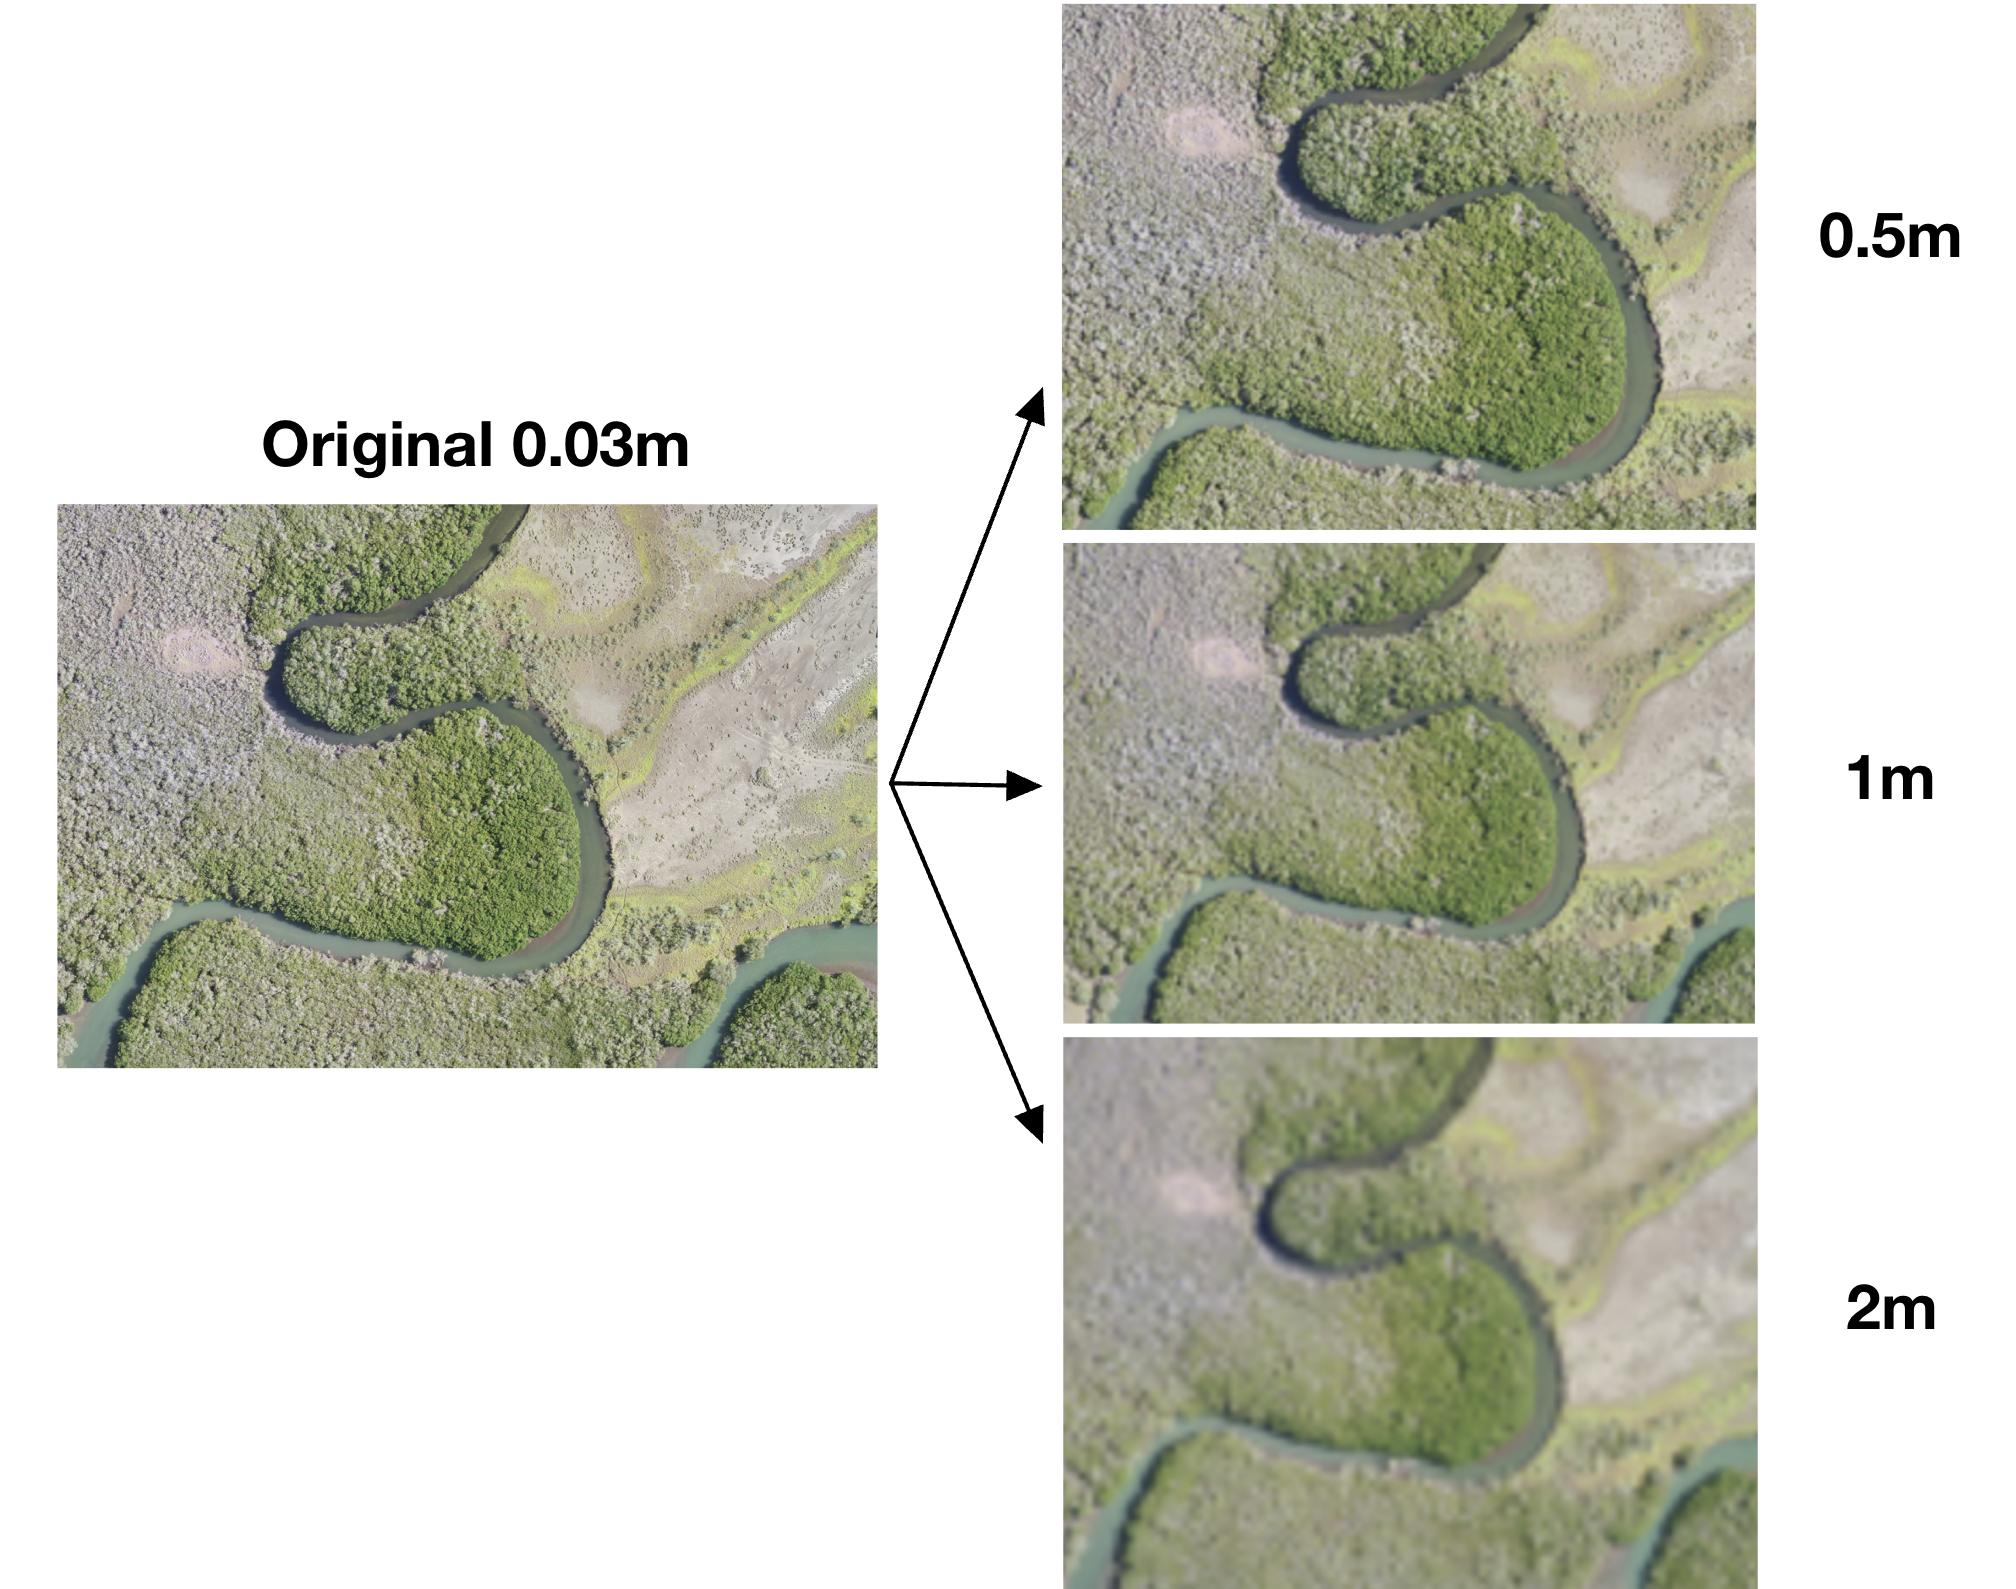
\includegraphics[height=0.7\textheight,width=0.7\textwidth,keepaspectratio]{images/Resampling.png}
\end{frame}

\begin{frame}{Results}
    \centering
    \includegraphics[height=0.7\textheight,width=0.7\textwidth,keepaspectratio]{images/og_multires_iou.png}
\end{frame}

\begin{frame}{Retraining Model on Multiple Resolutions}
    Adding resampled data to training dataset improves performance across the board.
    \centering
    \includegraphics[height=0.7\textheight,width=0.7\textwidth,keepaspectratio]{images/og_vs_multires.png}
\end{frame}

\begin{frame}{Performance for Super-resolution Target}
    Despite Gains in performance, the model is still not useful for 1m classification.
\centering
    \includegraphics[height=0.7\textheight,width=0.7\textwidth,keepaspectratio]{images/1m_metrics.png}
\end{frame}

\begin{frame}{Conclusion}
    Super-resolving from 10m to 1m will not be enough for our model.

    \begin{itemize}
        \item Possible Next Steps:
        \begin{enumerate}
            \item Build a super-res dataset from higher resolution satellites
            \item Collect labeled data for 1m imagery
            \item Give up on super-resolution
        \end{enumerate}
    \end{itemize}
\end{frame}